\chapter{Developer Documentation}
\label{chapter:DevDoc}

\section{Architectural Overview}
\label{sec:Arch}

Figure~\ref{fig:Arch} provides an overview of the system. The clang-plugin
developed produces a database for each translation-unit, which can then be
merged to make all variable declarations available to the frontend, which can
then suggest names for the variables.

The structure of the database can be seen in Figure~\ref{fig:Database}.

%Hack to get the stereo to be aligned next to the line instead of on it.
\newcommand{\stereorelation}[5]{
	#1[#3]{#4}{#5}
	#1[arg1=$\ll$#2$\gg$, pos1=0.5]{#4}{#5}
}

\begin{figure}
	\label{fig:Arch}
	\caption{Overview of Architectural Elements}
	\begin{center}
		\begin{tikzpicture}

			\umlclass[x=0, y=0]{header}{}{}
			\umlclass[x=0, y=-3]{source}{}{}
			\umlclass[x=5, y=-3]{clang}{}{}
			\umlclass[x=5, y=0]{plugin}{}{}
			\umlclass[x=10, y=0]{database}{}{}
			\umlclass[x=10, y=-3]{frontend}{}{}

			\stereorelation{\umlaggreg}
					{includes}{mult1=*, mult2=*}{source}{header}
			\stereorelation{\umluniassoc}
					{compiles}{mult1=1, mult2=*}{clang}{source}
			\stereorelation{\umluniassoc}
					{invokes}{mult1=1, mult2=1}{clang}{plugin}
			\stereorelation{\umluniassoc}
					{produces}{}{plugin}{database}
			\stereorelation{\umluniassoc}
					{loads}{mult1=1, mult2=*}{frontend}{database}

		\end{tikzpicture}
	\end{center}
\end{figure}

\begin{figure}
	\label{fig:Database}
	\caption{Structure of the Database}
	\begin{center}
		\begin{tikzpicture}
			\umlclass[x=0, y=0]{Database}{filename: string}{}
			\umlclass[x=5, y=0]{VariableDeclaration}{
				name: string \\
				type: string \\
				location: string
			}{}
			\umlclass[x=5, y=-5]{VariableOccurence}{
				location: string
			}

			\umlcompo[mult1=1, mult2=*]{Database}{VariableDeclaration}
			\umlcompo[mult1=1, mult2=*]{VariableDeclaration}{VariableOccurence}
		\end{tikzpicture}
	\end{center}
\end{figure}

\subsection{Database Format}
\label{sec:dbfmt}
The database produced by the compiler-plugin generates a list of declarations
that are later used for suggesting variables.
The database format is designed such that each translation unit creates its own
database, so that when a project is being built with a build-system that
supports incremental building, wherein a source change only causes the impacted
source file to be recompiled, the database produced for that source file can
then be recombined with the rest, to produced a complete overview of all
variables in the project. For a formal schema of the database, see
appendix \ref{appendix:schema}.

To support renaming of variables, we also need to track the location of any
references to the variables. This is to ensure that after renaming the
variable name at the point of declaration, we also must update every part of the
code that refers to this variable. This can not be achieved by mere textual
pattern-matching, as multiple scopes may have variables of the same name. This
means we have to list all occurences during analysis. When merging the databases
we also need to merge the list of occurences.

\section{Clang-plugin Architecture}

The clang-plugin contains all the code needed for traversing the Abstract
Syntax Tree, along with the routines needed for dumping the names that occur in
the codebase to a JSON file. All code in the clang-plugin is defined in
\lstinline|namespace dn|.

\subsection{Plugin}
The plugin first starts by loading \lstinline|Action| into
\lstinline|clang::FrontEndPluginRegistry|.

\begin{figure}[h]
	\label{fig:actionload}
	\caption{Loading the AST Action}
	\centering
	\begin{tikzpicture}
		\begin{umlpackage}{clang}
			\umlsimpleclass[x=0, y=0, width=6cm]{FrontendPluginRegistry}
		\end{umlpackage}
		\begin{umlpackage}{dn}
			\umlsimpleclass[x=0, y=-4, width=6cm]{ASTAction}
		\end{umlpackage}
		\stereorelation{\umluniassoc}{register}{mult1=1, mult2=1, name=register}
				{ASTAction}{FrontendPluginRegistry};
		\umlnote[x=+5, y=-2, width=8cm]{register-1}
				{\lstinline|FrontendPluginRegistry::Add<dn::Action> \_\{\}|}
	\end{tikzpicture}
\end{figure}

\subsection{Action}
\lstinline|Action| can then parse the
command-line arguments passed to Clang, so that it can deduce the filename that
was set for storing the output JSON. \lstinline|Action| uses
\lstinline|clang::PluginASTAction::ActionType Action::getActionType()| to inform
Clang that \lstinline|Action| should not inhibit compilation, and should be
invoked after the compilation has been done.

\begin{figure}[h]
	\label{fig:action}
	\caption{Action Collaboration Diagram}
	\centering
	\begin{tikzpicture}
		\begin{umlpackage}{clang}
			\umlclass[x=0, y=0, type=abstract]{PluginASTAction}{}{
				+\umlvirt{ASTConsumer* CreateASTConsumer($\ldots$)} \\
				+\umlvirt{bool ParseArgs($\ldots$)} \\
				+\umlvirt{ActionType getActionType()}
			}
		\end{umlpackage}
		\begin{umlpackage}{dn}
			\umlclass[x=0, y=-5]{Action}{
				- boost::optional<string> outputFilename
			}{
				+\umlvirt{ASTConsumer* CreateASTConsumer($\ldots$)} \\
				+\umlvirt{bool ParseArgs($\ldots$)} \\
				+\umlvirt{ActionType getActionType()}
			}
			\umlinherit{Action}{PluginASTAction}
			\umlsimpleclass[x=7.5, y=-5]{Consumer}
			\stereorelation{\umluniassoc}{creates}{mult1=1, mult2=1}
					{Action}{Consumer};
		\end{umlpackage}
	\end{tikzpicture}
\end{figure}

\subsection{Consumer}
Clang then loads the \lstinline|Consumer| as specifed by
\lstinline|Action::CreateASTConsumer|, which can then proceed with traversing
the Abstract Syntax Tree of the given Translation Unit.

\lstinline|Consumer|'s sole responsibility is to invoke the \lstinline|Visitor|
when invoked by Clang.

\begin{figure}[h]
	\label{fig:Consumer}
	\caption{Consumer Collaboration Diagram}
	\centering
	\begin{tikzpicture}
		\begin{umlpackage}{clang}
			\umlclass[x=0, y=0]{ASTConsumer}{}{
				+\umlvirt{void HandleTranslationUnit()}
			}
		\end{umlpackage}
		\begin{umlpackage}{dn}
			\umlclass[x=0, y=-5]{Consumer}{
				clang::CompilerInstance\& ci\\
				string inputFile \\
				string outputFile \\
				map<string, string> debugPrefixMap
			}{
				-\umlvirt{void HandleTranslationUnit()}
			}
			\umlsimpleclass[x=6.5, y=-5]{Visitor}
			\stereorelation{\umluniassoc}{calls}{mult1=1, mult2=1}
					{Consumer}{Visitor}
		\end{umlpackage}
		\umlinherit{Consumer}{ASTConsumer}
	\end{tikzpicture}
\end{figure}

\section{Implementation}
\subsection{Visiting the Abstract Syntax Tree}

There are two main tasks to accomplish when traversing the Abstract Syntax Tree:
the first is to record all variable declarations, the second is to record all
references to these variables.

Both of these tasks are accomplished by the \lstinline|Visitor| class.
To facilitate these tasks, Clang's \lstinline|RecursiveASTVisitor| provides two
functions for us to override: \lstinline|VisitDecl| and \lstinline|VisitStmt|.

A diagram of the involved classes can be seen in \fref{fig:Visitor}.

\begin{figure}[h]
	\label{fig:Visitor}
	\caption{Visitor Collaboration Diagram}
	\centering
	\begin{tikzpicture}
		\begin{umlpackage}{clang}
			\umlclass[x=0, y=0, template={Derived}]{RecursiveASTVisitor}{}{
				+\umlvirt{bool VisitDecl($\ldots$)} \\
				+\umlvirt{bool VisitDecl($\ldots$)}
			}
			\umlsimpleclass[x=6.8, y=0]{SourceLocation}
		\end{umlpackage}
		\begin{umlpackage}{dn}
			\umlclass[x=0, y=-6.5]{Visitor}{
				-string outputFile \\
				-map<string, string> debugPrefixMap \\
			}{
				+\umlvirt{bool VisitDecl($\ldots$)} \\
				+\umlvirt{bool VisitDecl($\ldots$)} \\
				+void printVariableNames($\ldots$) \\
				-void visitVariableDeclaration($\ldots$) \\
				-void visitFieldDeclaration($\ldots$) \\
				-void visitDecl$\ldots$ReferenceExpr$\ldots$($\ldots$) \\
				-void visitMemberExpression($\ldots$) \\
				-void addOccurence($\ldots$)
			}
			\umlclass[x=6.8, y=-6.5]{VariableDeclaration}{
				-string name \\
				-string type \\
				-vector<string> occurences
			}{
				+string getName() \\
				+string getType() \\
				+string getLocation($\ldots$) \\
				+bool operator==($\ldots$) \\
				+void addOccurence($\ldots$)
			}
			\umlcompo[mult1=1, mult2=*]{Visitor}{VariableDeclaration}
			\umlcompo[mult1=1, mult2=*]{VariableDeclaration}{SourceLocation}
		\end{umlpackage}
		\umlinherit{Visitor}{RecursiveASTVisitor}
	\end{tikzpicture}
\end{figure}

\lstinline|VisitDecl| is used to visit all declarations as described in
\fref{sec:visitdecl}, whereas \lstinline|VisitStmt| is used to visit all
statements as described in \fref{sec:visitstmt}.

\subsubsection{Visiting Declarations}
\label{sec:visitdecl}
There are two sorts of declarations that we are interested in: variable
declarations, and field declarations.

The kinds a variable declaration can be are as follows:
\begin{itemize}
	\item Function-local variable
	\item Global variable
	\item Function argument
\end{itemize}

Our task in all of these cases is to record the name, type and location of the
variable being declared. These are then used as a composite key to compare
variables. The location not only contains the line and column of the variable,
but also the filename. This is important as during the compilation of a
translation unit, we may also visit declarations that come from another file,
most notably header files. Once the databases are merged, duplicate variables
will be removed, as described in \fref{sec:dbmerge}.

\subsubsection{Visiting Statements}
\label{sec:visitstmt}
When visiting statements, most statements are of no use to us. The only types
of statements that are of interest to us, are statements that refer to variable
declarations (or field declarations). We record these references, so that when
renaming a variable, we know what other parts of the code we need to change.

When traversing statements, we only handle \lstinline|DeclRefExpr|s, and
\lstinline|MemberExpr|s.

In both cases, all we have to do is lookup the original declaration of the
variable (or field) that the expression refers to, and add the current source
location to its set of occurences. In most cases, the declaration will be
visited before the statement that refers to it, however there are two notable
exceptions.

The most obvious exception to this well-ordering is when we have a class that
has a member function that refers to a member of the class that is defined
before the member. In \CC{} the order of function definitions and members in a
class defintion does not matter like it normally would, and Clang traverses
these declarations and defintions roughly in the order they appear in the
source-code. This means we may occur a reference to a field before we have
managed to record the field itself.

The other --more subtle-- case where we may see a reference before a declaration
is in the case of template functions whose return type and signature are only
determined fully upon instantiation. These function templates needn't be
instantiated to be visited, however when they are, there arguments are
referenced before they are declared.

In both of the above cases, we need to make sure that the variable to which we
are trying to add an occurence already exists in the database. The naive
approach to this is to record it if it is not already present, and doing the
same when recording a declaration.

We cannot merely rely upon discovering all variable declarations by noticing
them through statements, as some variables are declared but never referred to.

\subsection{Merging the Databases}
\label{sec:dbmerge}

The database format as described in \fref{sec:dbfmt} was chosen to enable
merging the databases.
As the database is merely a list of Variables, each with a type, name location
and a list of occurences, these can be merged simply.
To support projects which may rename files during the lifetime of the project,
we ignore databases that refer to files that no longer exist. These databases
are referred to as stale.

Given a set of databases $input\_database_1, \ldots, input\_database_m$, we can
construct the set of non-stale databases as follows:
\begin{equation}
	database_1, \ldots, database_n = \left \{
		\substack {
			db \mid dn \in input\_database \\
			\land exists(input\_database.filename)
		}
	\right \}
\end{equation}
where $exists(filename)$ determines whether the file exists.

Given the following variable:
\begin{lstlisting}[mathescape, language=json, caption={Example Variable}]
{
	"type": TYPE,
	"name": NAME,
	"location": LOCATION,
	"occurences": [ $\ldots$ ]
}
\end{lstlisting}
and non-stale databases $database_1, \ldots, database_n$, we can construct the
merged variable as follows:

\begin{lstlisting}[escapeinside={(*}{*)}, language=json,
	caption={Merged Variable}]
{
	"type": TYPE,
	"name": NAME,
	"location": LOCATION,
	"occurences": [(*
		\[
			\bigcup_{i=1}^{n}{
				\left \{
					\substack{
						v.occurences \mid v \in database_i.variables \\
						\land v.type = TYPE \\
						\land v.name = NAME \\
						\land v.location = LOCATION
					}
				\right \}
			}
		\]
	*)
	]
}
\end{lstlisting}
Note that while the $input\_database_i$ each have filenames to determine
whether they are stale, the output of the merge process does not include this
field. This means that the merging operation is not associative, that is, merged
databases cannot be merged further.

\subsection{Making Suggestions}
\label{sec:suggesting}

When the developer requests a suggestion for a name, the first thing we need to
do is merge the databases that correspond to the project (as described in
\fref{sec:dbmerge}).

Once we have a merged database of all variables, we can then make a suggestion
based on the type of the variable we wish to rename.

\subsubsection{Making Suggestions Based on Type}

From the complete database $database$, we first get all the candidate names by
looking up all variables that have the same type as the variable we are
suggesting names for. Let's call the variable we are suggesting a new name for
$variable$. The set of names then becomes:

\[
	\left \{ v.name
			\mid v \in database.variables \land v.type = variable.type \right \}
\]
We also assign a weight to these names based on how frequently they occur.

\subsection{Renaming}

When renaming a variable, there are two main points at which to apply the
rename, the declaration of the variable (or field), and at all occurences.
This is implemented in the Python script \lstinline|suggest_names_rename|.

The first thing this script needs to do, is load and merge all the databases,
so that we can rename occurences of a variable located in a different file.

Care must be taken when there are multiple references to a variable in the same
line. If no two references occur in the same line, we can simply go to each
location and change the line and change the old name to the new name, changing
the length of the line as necessary. If there are multiple occurences in the
same line however, changing the occurences left-to-right would invalidate the
column index stores by the next occurence, so we have to perform each rename in
the same line right-to-left.
